\documentclass[compress]{beamer}

%--------------------------------------------------------------------------
% Common packages
%--------------------------------------------------------------------------
\usepackage[english]{babel}
\usepackage{pgfpages} % required for notes on second screen
\usepackage{graphicx}
\usepackage{subfigure}
\usepackage{multicol}
\usepackage[normalem]{ulem}

\usepackage{tabularx,ragged2e}
\usepackage{booktabs}
\usepackage{marvosym}

%--------------------------------------------------------------------------
% Load theme
%--------------------------------------------------------------------------
\usetheme{hri}

\usepackage{tikz}
\usetikzlibrary{patterns,shapes,fpu,fit,calc,mindmap,backgrounds,positioning,svg.path}

\tikzset{
  invisible/.style={opacity=0},
  visible on/.style={alt={#1{}{invisible}}},
  alt/.code args={<#1>#2#3}{%
    \alt<#1>{\pgfkeysalso{#2}}{\pgfkeysalso{#3}} % \pgfkeysalso doesn't change the path
  },
}

%% Neat trick to have only one navigation bullet per subsection
%% http://tex.stackexchange.com/questions/64333/one-navigation-bullet-per-subsection-with-subsection-false-in-custom-beamer-them
%\usepackage{etoolbox}
%\makeatletter
%\patchcmd{\slideentry}{\advance\beamer@xpos by1\relax}{}{}{}
%\def\beamer@subsectionentry#1#2#3#4#5{\advance\beamer@xpos by1\relax}%
%\makeatother
%%%%%%%%%%%%%%%%%%%%%%%%%%%%%%%%%%%%%%%

\graphicspath{{figs/}}

% for model of anthopomorphism
\newcommand{\IPA}{{$\mathcal{A}_0$~}}
\newcommand{\SLA}{{$\mathcal{A}_\infty$~}}
\newcommand{\sla}{{\mathcal{A}_\infty}}
\newcommand{\AntMax}{{$\mathcal{A}_{max}$~}}
\newcommand{\antMax}{{\mathcal{A}_{max}}}

% for HATP plans
\newcommand{\hatpaction}[3]{#1\\\textsf{\scriptsize #2,}\\\textsf{\scriptsize #3}}
\newcommand{\stmt}[1]{{\footnotesize \tt  #1}}

% for mutual modelling
\newcommand{\Mmodel}[3]{{\mathcal{M}(#1, #2, #3)}}
\newcommand{\model}[3]{{$\mathcal{M}(#1, #2, #3)$}}
\newcommand{\Model}[3]{{$\mathcal{M}^{\circ}(#1, #2, #3)$}}

% typeset logical concept
\newcommand{\concept}[1]{{\scriptsize \texttt{#1}}}

\newcommand{\backbutton}{\hfill\hyperlink{appendix}{\beamerreturnbutton{Supplementary material}}}
%--------------------------------------------------------------------------
% General presentation settings
%--------------------------------------------------------------------------
\title{\Large Socially-driven Autonomous Robots\newline for Real-World Human-Robot Interactions}
\subtitle{~}
\date{ISIR -- {\bf 06 Jan 2021}}
\author{Séverin Lemaignan}
\institute{Bristol Robotics Lab\\{\bf University of the West of England}}

%--------------------------------------------------------------------------
% Notes settings
%--------------------------------------------------------------------------
%\setbeameroption{show notes on second screen}
%\setbeameroption{hide notes}

\begin{document}


%%%%%%%%%%%%%%%%%%%%%%%%%%%%%%%%%%%%%%%%%%%%%%%%%%%%%%%%


%%%%%%%%%%%%%%%%%%%%%%%%%%%%%%%%%%%%%%%%%%%%%%%%%%%%%%%%

\maketitle

%%%%%%%%%%%%%%%%%%%%%%%%%%%%%%%%%%%%%%%%%%%%%%%%%%%%%%%%

\section*{Who Am I?}


{
    \fullbackground{europe_map}
    \begin{frame}[plain]
            \begin{tikzpicture}[>=latex, remember picture, overlay,
                input/.style={draw,circle, inner sep=0pt,minimum size=0.1cm}
                ]

                %\foreach \x in {-1, -0.9,..., 1}
                %    \foreach \y in {-1, -0.9,..., 1}
                %        \node[input] at (page cs:\x,\y){};

                \coordinate (kit) at (page cs:0.45,0.02);
                \coordinate (paris) at (page cs:0.2,0);
                \coordinate (paris2) at (page cs:0.23,-0.04);
                \coordinate (toulouse) at (page cs:0.1,-0.3);
                \coordinate (tum) at (page cs:0.55,0.05);
                \coordinate (epfl) at (page cs:0.38,-0.16);
                \coordinate (plym) at (page cs:-0.09,0.15);

                \node<2-3>[text width=5cm] at (page cs:-0.5,0.1) (msc) {\footnotesize Joint French (ParisTech) German (Karlsruhe Institute of Technology) MSc
                in \textbf{Mechanical Engineering}

                %\emph{top ten student out of 1000}
                };
                \node<3>[text width=5cm] at (page cs:-0.5,-0.22) (msc2)
                {\footnotesize MSc in \textbf{AI for Learning technologies} (Paris 5)
                
                %\emph{top student of the year}
                };

                \path<2-3>[->,ultra thick] (msc) edge (kit);
                \path<2-3>[->,ultra thick] (msc) edge (paris);
                \path<3>[->,ultra thick] (msc2) edge (paris2);

                \node<4>[text width=5cm] at (page cs:-0.5,0.0) (phd)
                {\footnotesize Joint French (CNRS LAAS) German (Technical University of Munich)
                PhD in \textbf{AI \& Cognitive Robotics}
                \vspace{1em}

                %\emph{Best 2012 CNRS PhD in Robotics}\\
                %\emph{PhD with High Distinction @TUM}
                };

                \path<4>[->,ultra thick] (phd) edge (toulouse);
                \path<4>[->,ultra thick] (phd) edge (tum);

                \node<5>[text width=5cm] at (page cs:-0.5,-0.1) (postdoc-epfl)
                {\footnotesize \textbf{Post-doc at EPFL}
                \vspace{1em}

                \emph{Supervision of the HRI team}\\
                \emph{Two main projects: CoWriter \& Cellulo}
                };

                \path<5>[->,ultra thick] (postdoc-epfl) edge (epfl);

                \node<6>[text width=5cm] at (page cs:-0.5,-0.1) (postdoc-plym)
                {\footnotesize \textbf{Post-doc at Plymouth University}
                \vspace{1em}

                \emph{EU Marie Skłodowska-Curie fellow} \\
                \emph{Social Cognition in Robotics}
                };

                \path<6>[->,ultra thick] (postdoc-plym) edge (plym);


            \end{tikzpicture}
    \end{frame}
}

\imageframe[color=black]{perso/robots}

%\begin{frame}{Academic Curriculum}
%    \begin{itemize}
%        \item<1-> Joint French (ParisTech) German (Karlsruhe Institute of Technology) MSc
%            in mechanical engineering
%            \begin{itemize}
%                \item \textbf{top ten student} out of 1000
%            \end{itemize}
%        \item<1-> MSc in AI for Learning technologies (University Paris 5)
%            \begin{itemize}
%                \item \textbf{top student} of the year
%            \end{itemize}
%        \item<2-> Joint French (CNRS LAAS) German (Technical University of Munich)
%            PhD in AI \& Cognitive Robotics
%            \begin{itemize}
%                \item \textbf{Best 2012 CNRS PhD in Robotics}
%                \item \textbf{High Distinction} in Germany
%            \end{itemize}
%
%    \end{itemize}
%
%
%\end{frame}

%\begin{frame}{Since my PhD}
%    2013--2015  \textbf{Post-doc at EPFL}
%    \begin{itemize}
%        \item<+-> built up a leading group in child-robot interaction
%        \item<+-> went up to 3 PhD + 3 MSc students
%        \item<+-> joint supervisions with Portugal, France
%        \item<+-> 2 high-visibility projects with large media coverage
%        \item<+-> 7 papers in 4 years at high-profile HRI conference, 2 awards
%    \end{itemize}
%
%    \onslide<6->
%    2015--2017 \textbf{EU Marie Skłodowska-Curie fellow} at Plymouth University on
%    \textbf{Theory of Mind} \& \textbf{Social cognition for robots}
%
%    \onslide<7->
%
%    \vspace{1em}
%    \large\centering
%    \textbf{50+ publications}; \textbf{900+ citations}; \textbf{H-index=15}
%
%\end{frame}




%%%%%%%%%%%%%%%%%%%%%%%%%%%%%%%%%%%%%%%%%%%%%%%%%%%%%%%%

\section*{Symbolic Social Cognition}


\imageframe{pr2-baby-3}

\note{
    \begin{itemize}
            \item Mix of geometry, time, semantics
            \item High geometric/temporal granularity (e.g. nodding)
            \item Lots of common-sense knowledge, cultural background
            \item Account for uncertainties
            \item Remember past experiences, predict future events
    \end{itemize}

}

\begin{frame}[plain]

    \centering
    {\bf Situated dialogue} effectively evidences the challenges

    \begin{columns}
        \begin{column}{0.5\linewidth}
            How can the robot make sense of and act upon a command like:
            \vspace{2em}

            \bf
            ``Can you give me that book?''
        \end{column}
        \begin{column}{0.5\linewidth}
            \begin{center}
                \includegraphics[width=\linewidth]{pr2-baby-3}
            \end{center}
        \end{column}
    \end{columns}

    \pause

    \vspace{2em}
    My PhD: a symbolic approach to this problem
\end{frame}


%%%%%%%%%%%%%%%%%%%%%%%%%%%%%%%%%%%%%%%%%%%%%%%%%%%%%%%%

{
    \paper{Lemaignan et al., {\bf Artificial Cognition for Social Human-Robot
    Interaction: An Implementation}, Artifical Intelligence, 2016}
\begin{frame}<3>[label=sitass]{Multi-modal Symbolic situation assessment}

    \begin{columns}
        \begin{column}{0.4\linewidth}
        \centering
        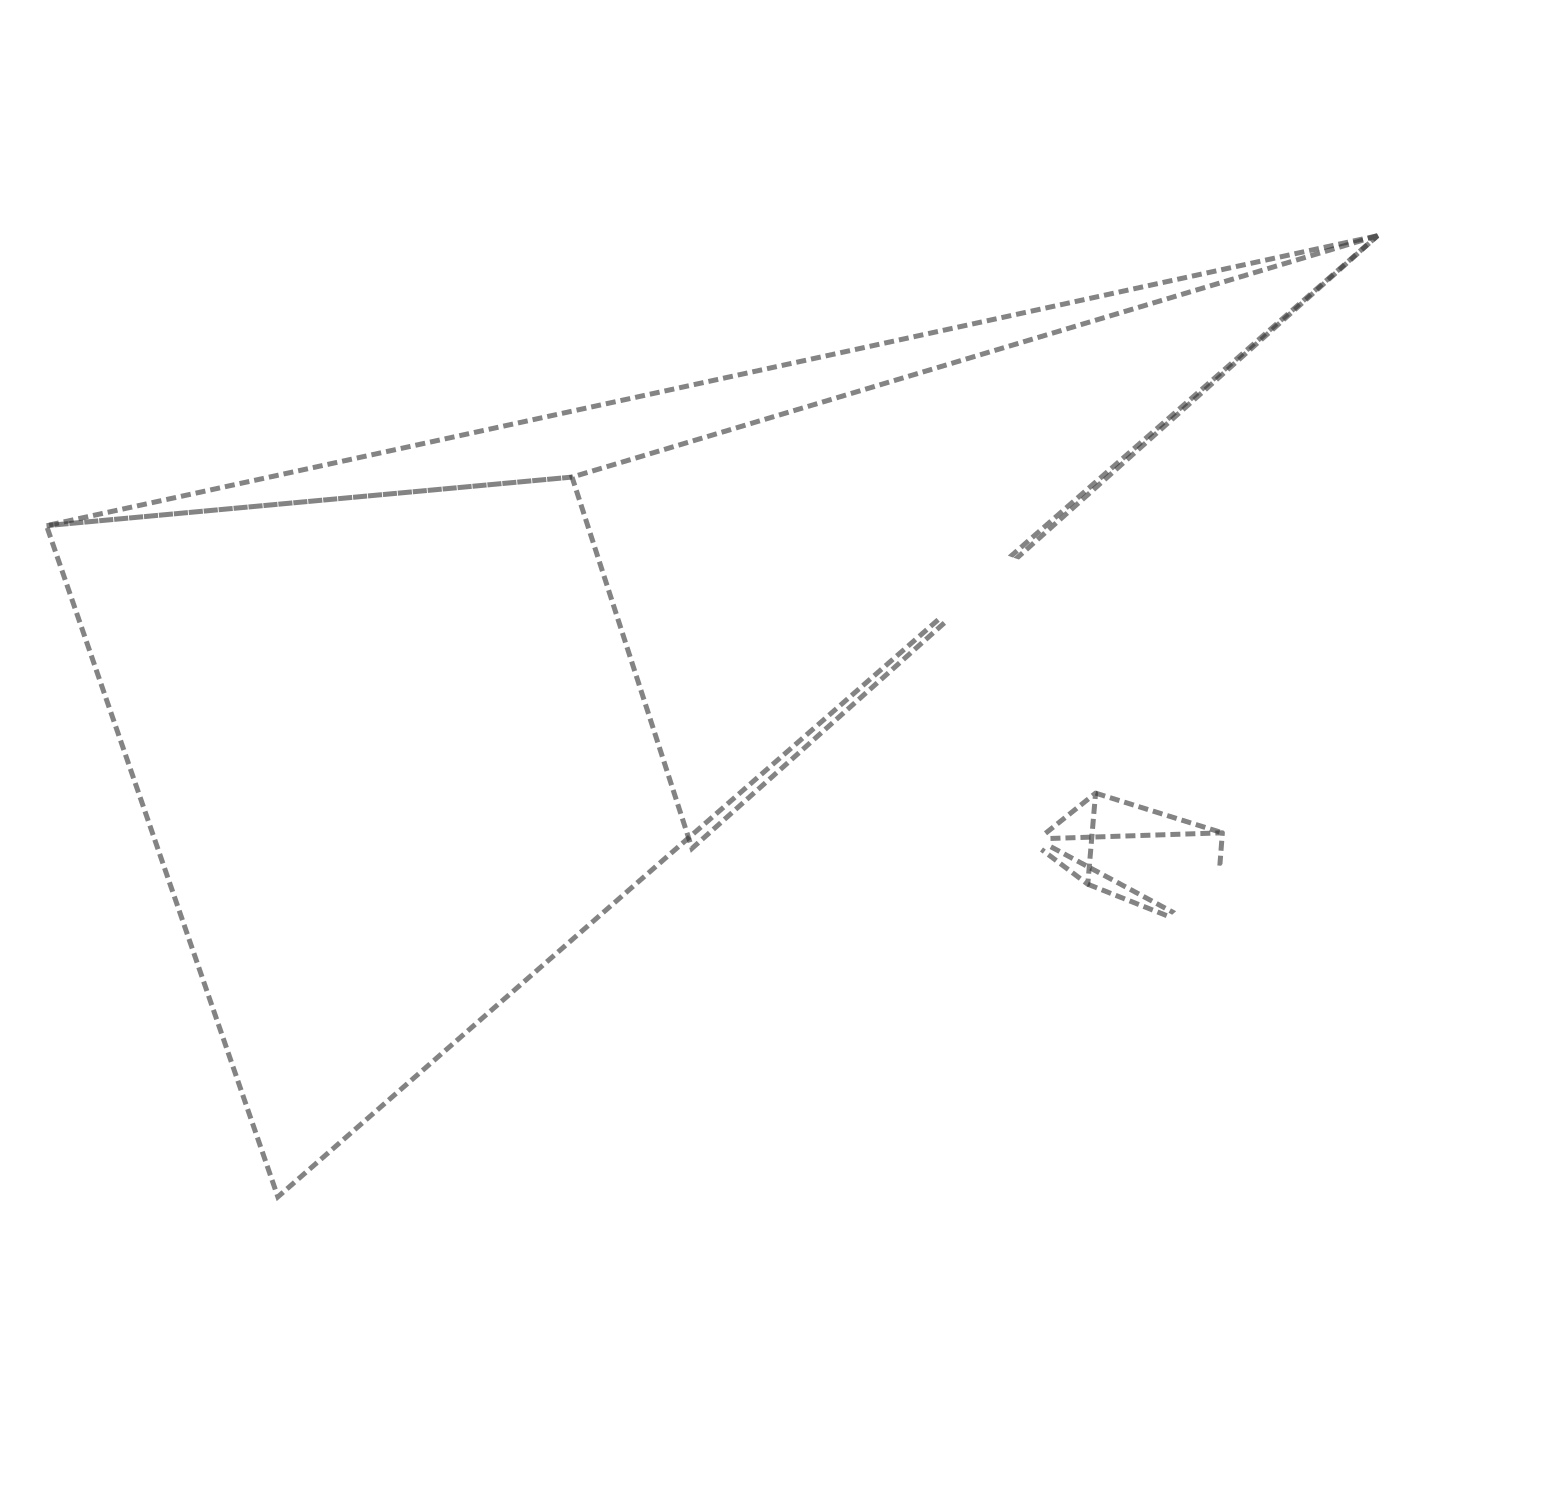
\includegraphics[width=\linewidth]{human-perspective-small}
             
        \end{column}
        \begin{column}{0.6\linewidth}
        
        \begin{figure}

        \resizebox{\columnwidth}{!}{%
        \begin{tikzpicture}[
            yscale=1.3,
            >=latex,
            every edge/.style={<-, draw, very thick},
            every node/.style={draw, font=\sf, node distance=0.5, rounded corners,
            align=center, inner sep=5pt,fill=hriSec2Dark!50},
            classof/.style={<-, draw=black!60, dashed},
            property/.style={<-, draw=hriSec2Comp},
            propname/.style={above, draw=none, fill=none, font=\tt, inner sep=2pt},
            instance/.style={draw=hriSec1Dark, font=\sf, node distance=0.5, rounded corners,
        align=center, inner sep=5pt, fill=none}]

            \node[fill=hriSec2Comp!50] (thing) {\textbf{thing}};
            \node [fill=hriSec3CompDark!50, node distance=1.8, below left=of
            thing](sthing) {place} edge[dashed] (thing);
            \node [fill=hriSec3CompDark!50, below left=of sthing] (agent) {agent} edge (sthing);
                \node [fill=hriSec3CompDark!50, below=of sthing] (artifact) {artifact} edge (sthing);
                \node [fill=hriSec3CompDark!50, below right=of sthing] (location) {physical
                support} edge (sthing);
                \node [fill=hriSec3CompDark!50, below right=of artifact] (table) {table}
                    edge (location) edge (artifact);


            \node [node distance=1, below right=of thing] (tthing) {temporal thing} edge (thing);
                \node [below right=of tthing] (evt) {event} edge[dashed] (tthing);
                            \node [below right=of evt] (act) {action} edge (evt);

        \uncover<2->{
        \draw[dotted, thick] (-8,-3.8) -- +(16, 0);

        \node [instance, below=3 of agent] (human) {human\_1} edge[classof, bend left] (agent);
        \node [instance, above left=of human] (human2) {human\_2} edge[classof, bend left] (agent);
        \node [instance, above right=of human, anchor=south] (robot) {myself} edge[classof, bend left] (agent);
        \node [instance, right=of human, anchor=north west] (book) {book\_game\_thrones}
        edge[classof] (artifact);
        \node [instance, right=2 of robot] (ikea) {ikea\_table} edge[classof, bend
        right] (table);
        \node [instance, right=2 of book] (brown) {brown} edge[property] node[propname] {hasColor} (book);


        }
        \uncover<3>{
        \draw[dotted, thick] (-8,-6.2) -- +(16, 0);

        \node [instance, below=5 of act] (moving) {move\_act\_42} edge[classof] (act);
        \path (moving.west) edge [property, out=180, in=-80, looseness=1] node[propname,below] {currentlyPerforms} (human.230);
        \path (human.280) edge [property, out=-80, in=-90, looseness=3.5] node[propname,right] {looksAt} (robot.south);
        \path (ikea.south) edge [property, out=-90, in=-80, looseness=2.5] node[propname, auto] {isOn} (book.320);
        }
        \end{tikzpicture}
        }

        \end{figure}

       \end{column}
    \end{columns}



        \badge{europe_phd}
\end{frame}
}

%%%%%%%%%%%%%%%%%%%%%%%%%%%%%%%%%%%%%%%%%%%%%%%%%%%%%%%%
%
%{
%\paper{Lemaignan et al. {\bf Grounding the Interaction: Anchoring
%Situated Discourse in Everyday HRI} Intl. J. of Social Robotics 2011}
%\begin{frame}{Dialogue Grounding}
%    \centering
%
%    I keep the NLP details for the questions, but:\\
%
%    \begin{columns}
%        \begin{column}{0.65\linewidth}
%
%    \centering
%    \vspace*{2em}
%    {\bf ``Give me the book on the table''}\\
%
%    \uncover<2-> {
%        $\downarrow$\\
%        {\tt me} $\rightarrow$ {\tt human\_1} \\
%        find({\tt\scriptsize ?obj type table}) $\rightarrow$ {\tt ikea\_table} \\
%        find({\tt\scriptsize ?obj type book, ?obj isOn ikea\_table})
%        $\rightarrow$ {\tt book\_game\_thrones} \\
%    }
%
%    \uncover<3-> {
%        $\downarrow$\\
%        { \tt
%            \textbf{human\_1} desires \textbf{give\_act\_1}, \\
%            \textbf{give\_act\_1} type \textbf{Give}, \\
%            \textbf{give\_act\_1} performedBy \textbf{myself}, \\
%            \textbf{give\_act\_1} actsOnObject \textbf{book}, \\
%            \textbf{give\_act\_1} receivedBy \textbf{human\_1} \\
%        }
%    }
%            
%        \end{column}
%        \begin{column}{0.35\linewidth}
%         \resizebox{\linewidth}{!}{%
% 
% 
%             \begin{tikzpicture}[
%                     >=latex,
%                 every edge/.style={draw, very thick},
%                 skill/.style={draw, rounded corners, align=center, inner sep=5pt, fill=black!20},
%                 label/.style={midway, align=center, font=\scriptsize, above},
%                 subpart/.style={rounded corners, draw, align=center, font=\scriptsize, fill opacity=0.5, text opacity=1, fill=white!50}]
% 
%             %%% PARSING
% 
%             \node at (0,0)[skill, fill=hriSec3CompDark!50] (prepro) {Pre-processing};
%                 \node [left=0.7 of prepro] (input) {\textbf{Input}};
%                 \path (input) edge [->] (prepro);
% 
%                 %\path (spark.100) edge [->, bend right] node[label] {symbolic \\ facts} (oro);
%                 \node [below =0.4 of prepro, skill, fill=hriSec3CompDark!50] (parsing) {Parsing};
%                 \path (prepro) edge [->] (parsing);
% 
%                 \coordinate (base-onto) at (4,0);
% 
%                 %%% RESOLUTION
%                     \node [below=0.4 of parsing, skill, fill=hriSec3!50, minimum height=4cm, minimum width=5cm] (resolution) {};
%                 \node [subpart, below=0.2 of resolution.115] (pron) {Pronouns \& \\ anaphora resolution};
%                 \node [subpart, below=0.2 of pron] (noun) {Noun phrase \\ resolution};
%                 \node [subpart, right=0.3 of noun, anchor=north west] (discr) {Discrimination};
%                 \node [subpart, below=0.2 of noun] (verb) {Verbal phrase \\ resolution};
%                 \node [subpart, cylinder, shape border rotate=90, aspect=0.5, below=0.2 of discr] (actions) {Actions};
%                 \path (pron) edge [->] (noun);
%                 \path (noun) edge [->] (discr);
%                 \path (noun) edge [->] (verb);
%                 \path (verb) edge [dashed, <->] (actions);
%                 \path (pron) edge [dashed, <->] node[label] {queries} (pron -| base-onto);
%                 \path (noun.20) edge [dashed, <->] node[label] {queries} (noun.20 -| base-onto);
%                 \path (discr) edge [<->] (discr -| base-onto);
% 
%                 \node [left=0.2 of resolution.west, rotate=90, anchor=south] {Resolution};
%                 \path (parsing) edge [->] (pron);
% 
%             %%% INTERPRETATION
%                     \node [skill, below=0.4 of resolution,minimum width=5cm, minimum height=3cm] (interp) {};
%                 \node [subpart, below=0.2 of interp.north] (content) {Content analysis};
%                 \node [below=0.6 of content.south west, subpart] (question) {Question \\ handler};
%                 \node [below=0.6 of content.south east, subpart] (stat) {Statement \\ builder};
%                 \path (content) edge [->] node[label, left] {question} (question);
%                 \path (content) edge [->] node [label, right] {goal | statement} (stat);
%                 \path (stat) edge [->] node [label] {asserts} (stat -| base-onto);
% 
%                 \node [left=0.2 of interp.west, rotate=90, anchor=south] {Interpretation};
% 
%                 \path (verb) edge [->] (content);
%                 \path (question) edge [dashed, bend right, <->] node[label] {queries} (question.south -| base-onto);
% 
%             %%% ONTOLOGY
%                     \node at (resolution.north -| base-onto) [rotate=-90, skill, minimum height=2cm, minimum width=7cm, fill=hriSec3!50, anchor=south west] (onto) {Ontology server};
% 
% 
%             %%% VERBALIZATION
%                 \node [below=0.7 of interp, skill, fill=hriSec2Dark!50] (verb) {Verbalization};
%             \path (question) edge [->] (verb);
%             \path (stat) edge [->] (verb);
%             \path (discr.south east) edge [black!50, dashed, bend left, <->] (verb.north east);
%             \node [right=0.7 of verb] (output) {\textbf{Output}};
%             \path (verb) edge [->] (output);
%         \end{tikzpicture}
%         }
%
%        \end{column}
%    \end{columns}
%
%        \badge{europe_phd}
%\end{frame}
%}
%
%%%%%%%%%%%%%%%%%%%%%%%%%%%%%%%%%%%%%%%%%%%%%%%%%%%%%%%%%
%
%{
%    \paper{Lemaignan et al., {\bf Artificial Cognition for Social Human-Robot
%    Interaction: An Implementation}, Artifical Intelligence, 2016}
%\begin{frame}{Multi-modal interaction}
%
%    \begin{columns}
%        \begin{column}{0.4\linewidth}
%        \centering
%        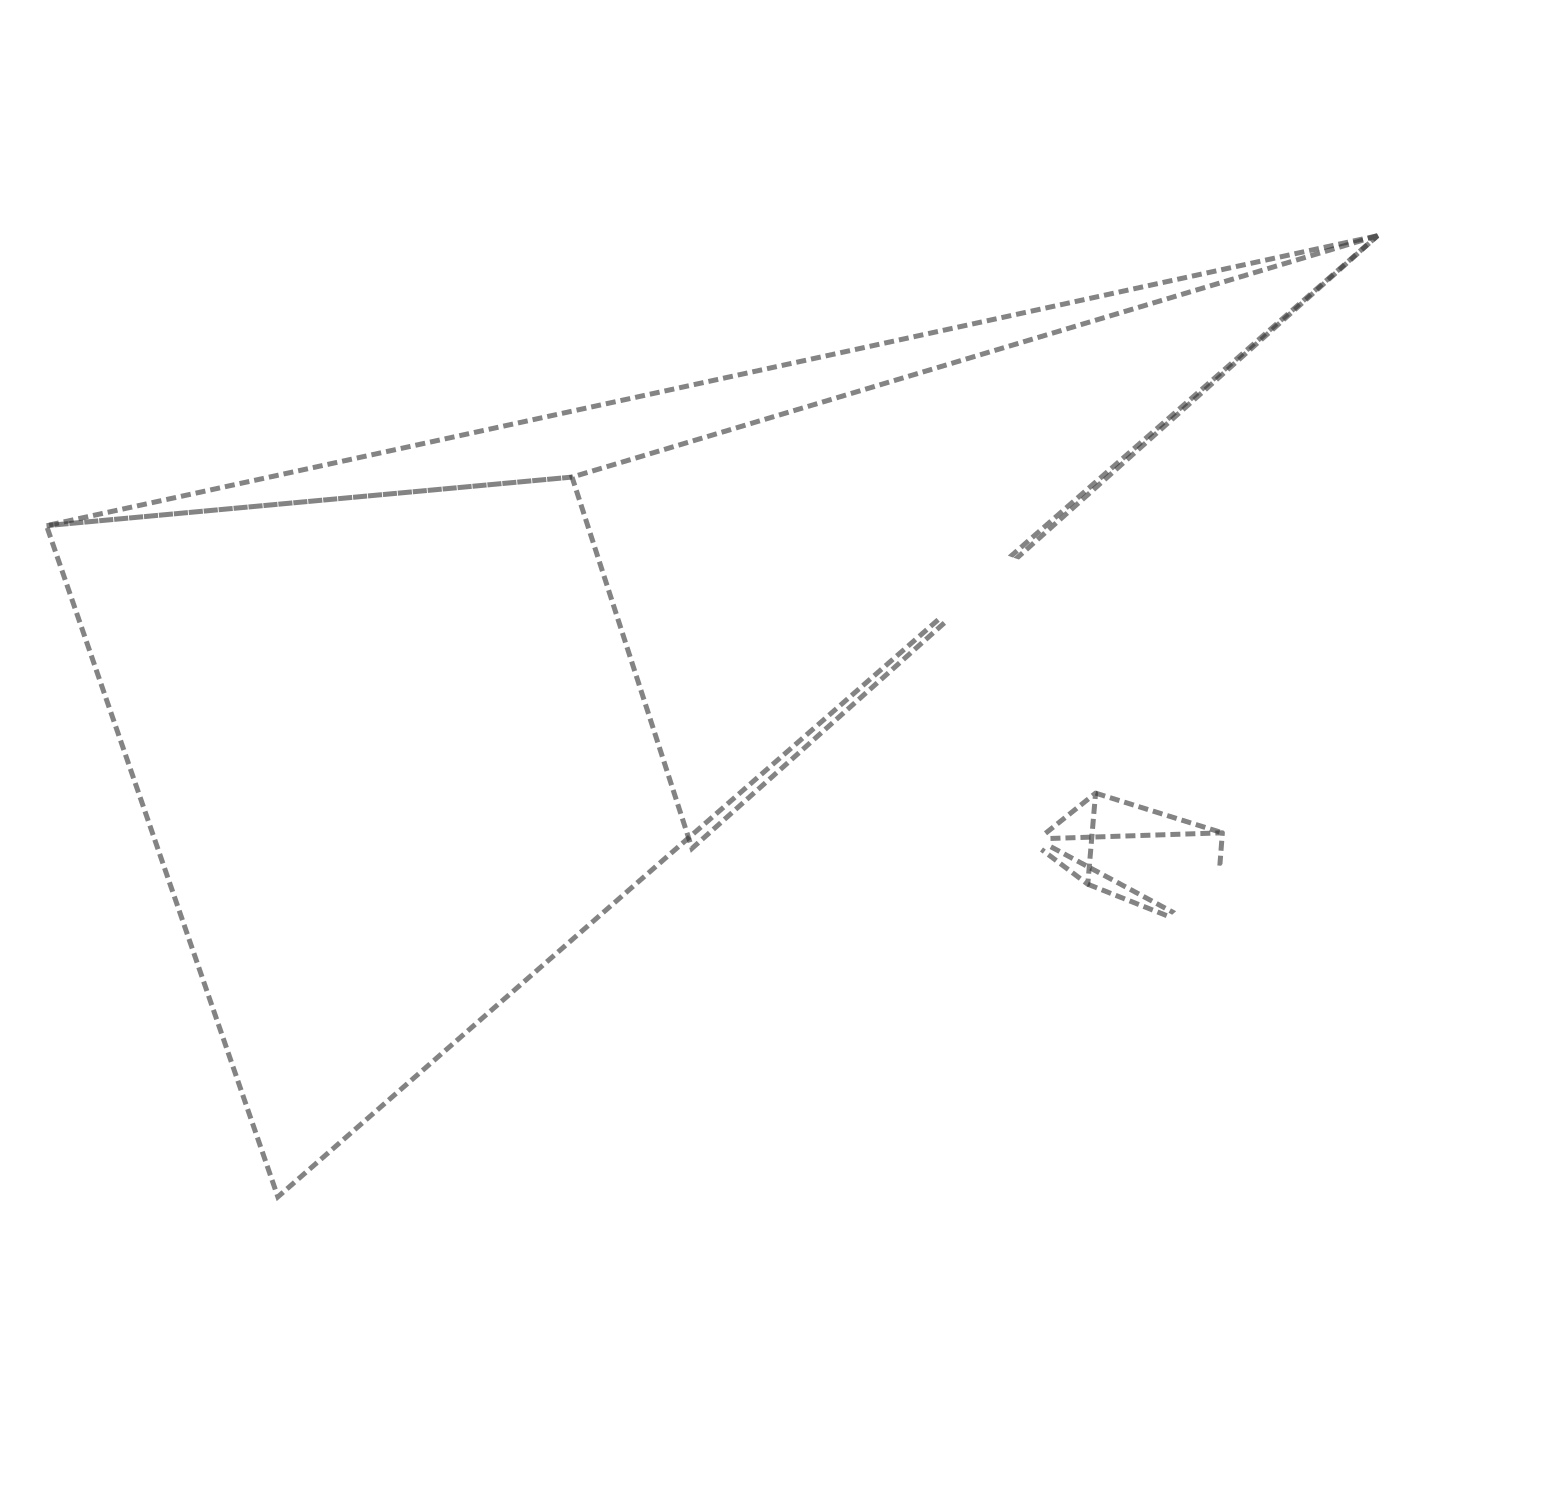
\includegraphics[width=\linewidth]{human-perspective-small}
%             
%        \end{column}
%        \begin{column}{0.6\linewidth}
%        
%    \centering
%    What about
%
%    {\bf ``Give me \emph{that} book''}?
%
%     \footnotesize
%    (or even: {\bf ``Give me \emph{that}!''})
%
%       \end{column}
%    \end{columns}
%
%
%
%        \badge{europe_phd}
%\end{frame}
%}

\videoframe[0.56]{videos/this_box.webm}
%\videoframe[0.56]{videos/this_box.webm?autostart&start=1}

\videoframe[0.7]{figs/cleantable/clean-table.webm}

%%%%%%%%%%%%%%%%%%%%%%%%%%%%%%%%%%%%%%%%%%%%%%%%%%%%%%%%
{
\paper{Lemaignan et al. {\bf Artificial Cognition for Social Human-Robot
     Interaction: An Implementation} Artifical Intelligence, 2016}
\begin{frame}{Full social \& autonomous interaction: one example}

    \begin{center}

     \begin{columns}
         \begin{column}{0.3\linewidth}
                 \includegraphics[height=0.75\paperheight]{clean-table}
         \end{column}
         \begin{column}{0.7\linewidth}
             \centering
             \resizebox{!}{0.75\paperheight}{%
                 \begin{tikzpicture}[
                         >=latex,
                     every edge/.style={draw, ultra thick, ->},
                     every node/.style={align=center},
                     robot/.style={fill=hriSec2Comp!50},
                     plan/.style={draw,
                      thick,  
                      circle, 
                      font=\sf,
                      align=center,
                      fill=hriSec3CompDark!50, 
                      minimum size=1cm, 
                      inner sep=0.1cm}
                  ]

                     \coordinate (figbottom) at (-0.5, -28.5);


                     \fill[gray!10!white] (4.6,.5) rectangle (figbottom);

                     \path (-0.5,0) edge (figbottom) node[sloped, above left, rotate=90] {\large\bf time};

                     \node at (2,0) (percept) {\bf Perception};
                     \node[below=0.5 of percept.south west, anchor=mid] {camera};
                     \node[below=0.5 of percept.south east, anchor=mid] {3D model};

                     \node[right=4 of percept, minimum width=2.5cm] (kb) {\bf Knowledge};
                     \node[below=0.5 of kb.south west, anchor=mid east] (kbr) {robot};
                     \node[below=0.5 of kb.south east, anchor=mid west] (kbh) {human};
                     \draw[dotted] (kbr) to (figbottom -| kbr);
                     \draw[dotted] (kbh) to (figbottom -| kbh);

                     \fill[gray!10!white] (12,.5) rectangle (17,0 |- figbottom);
                     \node[right=4.5 of kb] (plan) {\bf Plan};
                     \node[below=0.5 of plan.south west, anchor=mid east] (probot) {robot};
                     \node[below=0.5 of plan.south east, anchor=mid west] (phuman) {human};
                     \draw[dotted] (probot) to (figbottom -| probot);
                     \draw[dotted] (phuman) to (figbottom -| phuman);

                     \node[right=5 of plan] (action) {\bf Actions};
                     \node[below=0.5 of action.south west, anchor=mid east] (arobot) {robot};
                     \node[below=0.5 of action.south east, anchor=west] (ahuman) {human\\(monitoring)};
                     \draw[dotted] (arobot) to (figbottom -| arobot);
                     \draw[dotted] (ahuman) to (figbottom -| ahuman);

                     \draw[dashed] (-0.6,-1.2) --(24, -1.2);

                     \node[anchor=east] at (-0.5, -3) (t1) {\Large $t_1$};
                     \node[anchor=east, below=6 of t1] (t2) {\Large $t_2$};
                     \node[anchor=east, below=6 of t2] (t3) {\Large $t_3$};
                     \node[anchor=east, below=4 of t3] (t4) {\Large $t_4$};
                     \node[anchor=east, below=5 of t4] (t5) {\Large $t_5$};

                     %%%%%%%%%%%%%%%%%%%%%%%%%%%%%%%%%%%%%%%%%%%%%%%%%%%%%%%%%%%%%%%%%%%%%%%%%%%%%%%%%%%%%%%%%%%%
                     %%% PERCEPTIONS
                     %%%%%%%%%%%%%%%%%%%%%%%%%%%%%%%%%%%%%%%%%%%%%%%%%%%%%%%%%%%%%%%%%%%%%%%%%%%%%%%%%%%%%%%%%%%%

         \node at (t1 -| percept) (cam1) {\includegraphics[height=2cm]{cleantable/manip_run_cam1.png}};
         \node at (t2 -| percept) (cam2) {\includegraphics[height=2cm]{cleantable/manip_run_cam2.png}};
         \node at (t3 -| percept) (cam3) {\includegraphics[height=2cm]{cleantable/manip_run_cam3.png}};
         \node at (t4 -| percept) (cam4) {\includegraphics[height=2cm]{cleantable/manip_run_cam4.png}};
         \node at (t5 -| percept) (cam5) {\includegraphics[height=2cm]{cleantable/manip_run_cam5.png}};

         %%%%%%%%%%%%%%%%%%%%%%%%%%%%%%%%%%%%%%%%%%%%%%%%%%%%%%%%%%%%%%%%%%%%%%%%%%%%%%%%%%%%%%%%%%%%
         %%% KNOWLEDGE
         %%%%%%%%%%%%%%%%%%%%%%%%%%%%%%%%%%%%%%%%%%%%%%%%%%%%%%%%%%%%%%%%%%%%%%%%%%%%%%%%%%%%%%%%%%%%

         \node[fill=white,align=left] at (cam1 -| kbr) (kb1) {\stmt{TAPE isVisible true}\\
                                                    \stmt{TAPE isReachable true}\\
                                                    \stmt{TAPE isOn TABLE}\\
                                                    \stmt{BIN isVisible true}\\
                                                    \stmt{BIN isReachable false}};

         \node[fill=white,align=left] at (cam1 -| kbh) {\stmt{TAPE isVisible true}\\
                                                    \stmt{TAPE isReachable false}\\
                                                    \stmt{TAPE isOn TABLE}\\
                                                    \stmt{BIN isVisible true}\\
                                                    \stmt{BIN isReachable true}};

         \node[fill=white,align=left] at (cam2 -| kbr) (kb2) {\stmt{ROBOT hasInHand TAPE}};


         \node[fill=white,align=left] at (cam3 -| kbr) {\stmt{TAPE isReachable true}\\
                                        \stmt{TAPE isVisible true} \\
                                        \stmt{TAPE isOn TABLE}};

         \node[fill=white,align=left ] at (cam3 -| kbh) (kb3) {\stmt{TAPE isReachable true}\\
                                         \stmt{TAPE isVisible true}};

         \node[fill=white,align=left] at (cam4 -| kbh) (kb4) {\stmt{HUMAN hasInHand TAPE}};

         \node[fill=white,align=left] at (cam5 -| kbr)  {\stmt{TAPE isIn BIN}};
         \node[fill=white,align=left] at (cam5 -| kbh) (kb5) {\stmt{TAPE isIn BIN}};

         %%%%%%%%%%%%%%%% %%%%%%%%%%%%%%%%%%%%%%%%%%%%%%%%%%%%%%%%%%%%%%%%%%%%%%%%%%%%%%%%%%%%%%%%%%%%
         %%% PLANS
         %%%%%%%%%%%%%%%%%%%%%%%%%%%%%%%%%%%%%%%%%%%%%%%%%%%%%%%%%%%%%%%%%%%%%%%%%%%%%%%%%%%%%%%%%%%%

         \node[fill=gray!10!white,below=1 of plan] (incoming) {\bf \Large Incoming goal \\ \it Clean the table!};

         \node[anchor=north, plan, robot] at (cam1.south -| probot) (pr1) {\bf TAKE\\TAPE\\TABLE};
         \node[anchor=north, plan, robot] at (cam2.south -| probot)  (pr2) {\bf PUTRV\\TAPE\\TABLE} edge[<-] (pr1);
         \node[anchor=north, plan] at (cam3.south -| phuman) (ph1) {\bf TAKE\\TAPE\\TABLE} edge[<-] (pr2);
         \node[anchor=north, plan]  at (cam4.south -| phuman) (ph2) {\bf PUT\\TAPE\\BIN} edge[<-] (ph1);

         \node[fill=gray!10!white,anchor=north] at (cam5.south -| plan) (done) {\bf \Large Goal completed};

         %%%%%%%%%%%%%%%%%%%%%%%%%%%%%%%%%%%%%%%%%%%%%%%%%%%%%%%%%%%%%%%%%%%%%%%%%%%%%%%%%%%%%%%%%%%%
         %%% ACTIONS
         %%%%%%%%%%%%%%%%%%%%%%%%%%%%%%%%%%%%%%%%%%%%%%%%%%%%%%%%%%%%%%%%%%%%%%%%%%%%%%%%%%%%%%%%%%%%

         \only{
             \node[fill=white] at (pr1 -| arobot) (ep1) {\it evaluate pre-conditions};

         \node[below=0.1 of ep1] (mhp1) {%
             \begin{tikzpicture}
                 \node[fill=white] (title) {\bf motion planning};
                 \node[below=0.1 of title.south west, label=below:{\tt PICK\_GOTO}] (mapg) {\includegraphics{cleantable/MHP_ARM_PICK_GOTO}};
                 \node[fill=white,right=of mapg, label=below:{\tt TAKE\_TO\_FREE}] (mattf) {\includegraphics{cleantable/MHP_ARM_TAKE_TO_FREE}} edge[<-] (mapg);
             \end{tikzpicture}
         };
         \node[fill=white,below=0.1 of mhp1] (me1) {\bf motion execution};
         \node[fill=white,below=0.1 of me1] (ae1) {\it assess post-conditions};
     }
     %%%%%%%%%%%%%%%%%%%%%%%%%%%%%%%%%%%%%%%%%%%%%%%%%%%%%%%%%%%%%%%%%%%%%%%%%%%%%%%%%%%%%%%%%%%%%
         \only{
             \node[fill=white] at (pr2 -| arobot) (ep2) {\it evaluate pre-conditions};

         \node[below=0.1 of ep2] (mhp2) {%
             \begin{tikzpicture}
                 \node[fill=white] (title) {\bf motion planning};
                 \node[fill=white,below=0.1 of title, label=below:{\tt ESCAPE}] (maeo) {\includegraphics{cleantable/MHP_ARM_ESCAPE_OBJECT}};
                 \node[left=of maeo, label=below:{\tt PLACE\_FROM\_FREE}] (mapff) {\includegraphics{cleantable/MHP_ARM_PLACE_FROM_FREE}} edge (maeo);
                 \node[fill=white,right=of maeo, label=below:{\tt TO\_FREE}] (maf) {\includegraphics{cleantable/MHP_ARM_FREE}} edge[<-] (maeo);
             \end{tikzpicture}
         };
         \node[fill=white,below=0.1 of mhp2] (me2) {\bf motion execution};
         \node[fill=white,below=0.1 of me2] (ae2) {\it assess post-conditions};
     }
     %%%%%%%%%%%%%%%%%%%%%%%%%%%%%%%%%%%%%%%%%%%%%%%%%%%%%%%%%%%%%%%%%%%%%%%%%%%%%%%%%%%%%%%%%%%%%

         \node[anchor=north] at (ph1 -| ahuman) (wait1) {%
             \begin{tikzpicture}
                 \node[fill=white] (title) {\it wait for pick\\ {\tt TAPE} \it from {\tt TABLE}};
                 \node[below=0.1 of title] {\includegraphics{cleantable/wait_for_pick}};
             \end{tikzpicture}
         };

         \node[anchor=north] at (ph2 -| ahuman) (wait2) {%
             \begin{tikzpicture}
                 \node[fill=white] (title) {\it wait for put\\ {\tt TAPE} \it into {\tt BIN}};
                 \node[below=0.1 of title] {\includegraphics{cleantable/wait_for_throw}};
             \end{tikzpicture}
         };


         %%%%%%%%%%%%%%%%%%%%%%%%%%%%%%%%%%%%%%%%%%%%%%%%%%%%%%%%%%%%%%%%%%%%%%%%%%%%%%%%%%%%%%%%%%%%
         %%% FLOW
         %%%%%%%%%%%%%%%%%%%%%%%%%%%%%%%%%%%%%%%%%%%%%%%%%%%%%%%%%%%%%%%%%%%%%%%%%%%%%%%%%%%%%%%%%%%%
         \draw[dotted, ->, in=45, out=180] (incoming.west) to (kb1);
         \draw[dotted, ->, bend right] (kb1) to (pr1);
         \draw[dotted, ->, bend left] (pr1) to (ep1);
         \draw[dotted, ->, in=45, out=180] (ae1.west) to (kb2);
         \draw[dotted, ->, bend right] (kb2) to (pr2);
         \draw[dotted, ->, bend left] (pr2) to (ep2);
         \draw[dotted, ->, in=45, out=180] (ae2.west) to (kb3);
         \draw[dotted, ->, bend right] (kb3) to (ph1);
         \draw[dotted, ->, bend left] (ph1) to (wait1);
         \draw[dotted, ->, in=-20, out=180] (wait1.west) to (kb4.east);
         \draw[dotted, ->, bend right] (kb4) to (ph2);
         \draw[dotted, ->, bend left] (ph2) to (wait2);
         \draw[dotted, ->, in=20, out=180] (wait2.west) to (kb5);
         \draw[dotted, ->, bend left] (kb5.east) to (done.north);


     \end{tikzpicture}
      }
         \end{column}
     \end{columns}
    \end{center}

\end{frame}
}

%%%%%%%%%%%%%%%%%%%%%%%%%%%%%%%%%%%%%%%%%%%%%%%%%%%%%%%%%
%
%\section{One step further: Theory of Mind}
%
%%%%%%%%%%%%%%%%%%%%%%%%%%%%%%%%%%%%%%%%%%%%%%%%%%%%%%%%%

\begin{frame}[plain]

    \begin{center}
        \includegraphics[width=0.8\linewidth]{videos/this_box_thumb}

        What if I ask for the object in the box, but the robot has
        moved it somewhere else?


    \pause

        {\bf False-belief situation}
    \end{center}
\end{frame}

%%%%%%%%%%%%%%%%%%%%%%%%%%%%%%%%%%%%%%%%%%%%%%%%%%%%%%%%%

{
\paper{Ros, Lemaignan et al., {\bf Which One? Grounding the Referent Based on Efficient HRI}, ROMAN 2010}
\begin{frame}{Parallel Models: towards a theory of mind}
        \begin{multicols}{2}
            \begin{figure}
                \resizebox{0.4\textwidth}{!}{
                    \begin{tikzpicture}[
                        >=latex,
                        every edge/.style={<-, draw, very thick},
                        every node/.style={draw, font=\sf, node distance=0.5, rounded corners,
                                        align=center, inner sep=5pt,fill=hriSec2Dark!50},
                        classof/.style={<-, draw=black!60, dashed},
                        property/.style={<-, draw=hriSec2Comp},
                        propname/.style={above, draw=none, fill=none, font=\tt, inner sep=2pt},
                        instance/.style={draw=hriSec1Dark, font=\sf, node distance=0.5, rounded corners,
                        align=center, inner sep=5pt, fill=white}]

                    \node[fill=hriSec2Comp!50] (thing) {\textbf{thing}};
                    \node [fill=hriSec3CompDark!50, node distance=1.8, below left=of thing](sthing) {place} edge[dashed] (thing);
                    \node [fill=hriSec3CompDark!50, below left=of sthing] (agent) {agent} edge (sthing);
                        \node [fill=hriSec3CompDark!50, below=of sthing] (artifact) {artifact} edge (sthing);
                        \node [fill=hriSec3CompDark!50, below right=of sthing] (location) {physical
                        support} edge (sthing);
                        \node [fill=hriSec3CompDark!50, below right=of artifact] (table) {table}
                            edge (location) edge (artifact);


                    \node [node distance=1, below right=of thing] (tthing) {temporal thing} edge (thing);
                        \node [below right=of tthing] (evt) {event} edge[dashed] (tthing);
                                    \node [below right=of evt] (act) {action} edge (evt);

                \draw[dotted, thick] (-7,-5) -- (7.5, -5);

                \node [instance, below=3 of agent] (human) {human\_1} edge[classof, bend left] (agent);
                \node [instance, above left=of human] (human2) {human\_2} edge[classof, bend left] (agent);
                \node [instance, above right=of human, anchor=south] (robot) {pr2\_robot} edge[classof, bend left] (agent);
;
                \node [instance, right=of human, anchor=north west] (book) {book\_game\_thrones}
                edge[classof] (artifact);
                \node [instance, right=3 of robot] (ikea) {ikea\_table} edge[classof, bend
                right] (table);
                \node [instance, right=2 of book] (red) {red} edge[property] node[propname] {hasColor} (book);

                \node<2> [instance,right=1 of robot,fill=hriSec2] {myself} edge[property] node[propname, auto,above] {$\equiv$} (robot);

                \draw[dotted, thick] (-7,-8) -- (7.5, -8);

                \path (book.200) edge [property, out=-100, in=-80, looseness=2]
                node[propname,auto] {isNextTo} (human.south);
                \path (book.270) edge [property, out=-100, in=-90, looseness=3.5] node[propname,auto] {looksAt} (robot.south);
                \path (ikea.south) edge [property, out=-90, in=-80, looseness=3] node[propname, auto] {isOn} (book.320);
                \end{tikzpicture}
            }

            \end{figure}
            \begin{figure}
                \resizebox{0.4\textwidth}{!}{
                    \begin{tikzpicture}[
                        >=latex,
                        every edge/.style={<-, draw, very thick},
                        every node/.style={draw, font=\sf, node distance=0.5, rounded corners,
                                        align=center, inner sep=5pt,fill=hriSec2Dark!50},
                        classof/.style={<-, draw=black!60, dashed},
                        property/.style={<-, draw=hriSec2Comp},
                        propname/.style={above, draw=none, fill=none, font=\tt, inner sep=2pt},
                        instance/.style={draw=hriSec1Dark, font=\sf, node distance=0.5, rounded corners,
                        align=center, inner sep=5pt, fill=white}]

                    \node[fill=hriSec2Comp!50] (thing) {\textbf{thing}};
                    \node [fill=hriSec3CompDark!50, node distance=1.8, below left=of thing](sthing) {place} edge[dashed] (thing);
                    \node [fill=hriSec3CompDark!50, below left=of sthing] (agent) {agent} edge (sthing);
                        \node [fill=hriSec3CompDark!50, below=of sthing] (artifact) {artifact} edge (sthing);
                        \node [fill=hriSec3CompDark!50, below right=of sthing] (location) {physical
                        support} edge (sthing);
                        \node [fill=hriSec3CompDark!50, below right=of artifact] (table) {table}
                            edge (location) edge (artifact);


                    \node [node distance=1, below right=of thing] (tthing) {temporal thing} edge (thing);
                        \node [below right=of tthing] (evt) {event} edge[dashed] (tthing);
                                    \node [below right=of evt] (act) {action} edge (evt);

                \draw[dotted, thick] (-7,-5) -- (7.5, -5);

                \node [instance, below=3 of agent] (human) {human\_1} edge[classof, bend left] (agent);
                \node [instance, above left=of human] (human2) {human\_2} edge[classof, bend left] (agent);
                \node [instance, above right=of human, anchor=south] (robot) {pr2\_robot} edge[classof, bend left] (agent);
;
                \node [instance, right=of human, anchor=north west] (book) {book\_game\_thrones}
                edge[classof] (artifact);
                \node [instance, right=3 of robot] (ikea) {ikea\_table} edge[classof, bend
                right] (table);
                \node [instance, right=2 of book] (red) {red} edge[property] node[propname] {hasColor} (book);

                \node<2> [instance,below left=1 of human,fill=hriSec2] {myself} edge[property] node[propname, auto,above] {$\equiv$} (human);

                \draw[dotted, thick] (-7,-8) -- (7.5, -8);

                \path (book.200) edge [property, out=-100, in=-80, looseness=2]
                node[propname,auto] {isNextTo} (human.south);
                \path (book.270) edge [property, out=-100, in=-90, looseness=3.5] node[propname,auto] {looksAt} (robot.south);
                \path (ikea.south) edge [property, out=-90, in=-80, looseness=3] node[propname, auto] {isOn} (book.320);
                \end{tikzpicture}
            }
            \end{figure}
            \begin{figure}
                \resizebox{0.4\textwidth}{!}{
                    \begin{tikzpicture}[
                        >=latex,
                        every edge/.style={<-, draw, very thick},
                        every node/.style={draw, font=\sf, node distance=0.5, rounded corners,
                                        align=center, inner sep=5pt,fill=hriSec2Dark!50},
                        classof/.style={<-, draw=black!60, dashed},
                        property/.style={<-, draw=hriSec2Comp},
                        propname/.style={above, draw=none, fill=none, font=\tt, inner sep=2pt},
                        instance/.style={draw=hriSec1Dark, font=\sf, node distance=0.5, rounded corners,
                        align=center, inner sep=5pt, fill=white}]

                    \node[fill=hriSec2Comp!50] (thing) {\textbf{thing}};
                    \node [fill=hriSec3CompDark!50, node distance=1.8, below left=of thing](sthing) {place} edge[dashed] (thing);
                    \node [fill=hriSec3CompDark!50, below left=of sthing] (agent) {agent} edge (sthing);
                        \node [fill=hriSec3CompDark!50, below=of sthing] (artifact) {artifact} edge (sthing);
                        \node [fill=hriSec3CompDark!50, below right=of sthing] (location) {physical
                        support} edge (sthing);
                        \node [fill=hriSec3CompDark!50, below right=of artifact] (table) {table}
                            edge (location) edge (artifact);


                    \node [node distance=1, below right=of thing] (tthing) {temporal thing} edge (thing);
                        \node [below right=of tthing] (evt) {event} edge[dashed] (tthing);
                                    \node [below right=of evt] (act) {action} edge (evt);

                \draw[dotted, thick] (-7,-5) -- (7.5, -5);

                \node [instance, below=3 of agent] (human) {human\_1} edge[classof, bend left] (agent);
                \node [instance, above left=of human] (human2) {human\_2} edge[classof, bend left] (agent);
                \node [instance, above right=of human, anchor=south] (robot) {pr2\_robot} edge[classof, bend left] (agent);
;
                \node [instance, right=of human, anchor=north west] (book) {book\_game\_thrones}
                edge[classof] (artifact);
                \node [instance, right=3 of robot] (ikea) {ikea\_table} edge[classof, bend
                right] (table);
                \node [instance, right=2 of book] (red) {red} edge[property] node[propname] {hasColor} (book);

                \node<2> [instance,below=1 of human2,fill=hriSec2] {myself} edge[property] node[propname, auto] {$\equiv$} (human2);

                \draw[dotted, thick] (-7,-8) -- (7.5, -8);

                \path (book.200) edge [property, out=-100, in=-80, looseness=2]
                node[propname,auto] {isNextTo} (human.south);
                \path (book.270) edge [property, out=-100, in=-90, looseness=3.5] node[propname,auto] {looksAt} (robot.south);
                \path (ikea.south) edge [property, out=-90, in=-80, looseness=3] node[propname, auto] {isOn} (book.320);
                \end{tikzpicture}
            }
            \end{figure}
            {\vspace*{1.5cm}\hspace*{2.5cm}\huge...}
        \end{multicols}
        \badge{europe_phd}
\end{frame}
}

%%%%%%%%%%%%%%%%%%%%%%%%%%%%%%%%%%%%%%%%%%%%%%%%%%%%%%%%

\videoframe[0.56]{videos/dialogs.webm}
%\videoframe[0.56]{videos/dialogs.webm?autostart}


\section*{On the field}

%%%%%%%%%%%%%%%%%%%%%%%%%%%%%%%%%%%%%%%%%%%%%%%%%%%%%%%%

\imageframe[color=black]{experiments}

\begin{frame}{Experimental work}

        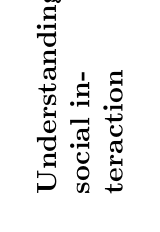
\begin{tikzpicture}
            \node[rotate=90,text width=2cm]{\textbf{Understanding\\ social interaction}};
        \end{tikzpicture}
            \hyperlink{croquignole}{\includegraphics[height=0.2\paperheight]{ranger/croquignole-single}}
            \hspace{0.5em}
            \hyperlink{dominos}{\includegraphics[height=0.2\paperheight]{ranger/domino-mistake}}
            \hspace{0.5em}
            \hyperlink{anthropomorphism}{\includegraphics[height=0.2\paperheight]{dynamics_anthropo}}

        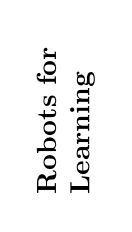
\begin{tikzpicture}
            \node[rotate=90,text width=2cm]{\textbf{Robots for \\Learning}};
        \end{tikzpicture}
            \hyperlink{cellulo}{\includegraphics[height=0.2\paperheight]{cellulo/concept-solar-system}}
            \hspace{0.5em}
            \hyperlink{cowriter-impl}{\includegraphics[height=0.2\paperheight]{cowriter/pca}}

        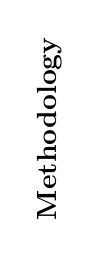
\begin{tikzpicture}
            \node[rotate=90]{\textbf{Methodology}};
        \end{tikzpicture}
            \hyperlink{withmeness}{\includegraphics[height=0.2\paperheight]{withmeness/withmeness}}
            \hspace{0.5em}
            \hyperlink{asr}{\includegraphics[height=0.2\paperheight]{speech-reco/record_img}}
            \hspace{0.5em}
            \hyperlink{constructs}{\includegraphics[height=0.2\paperheight]{ranger/questionnaire}}

\end{frame}

%%%%%%%%%%%%%%%%%%%%%%%%%%%%%%%%%%%%%%%%%%%%%%%%%%%%%%%%

\imageframe[color=black]{cowriter/henry}

%%%%%%%%%%%%%%%%%%%%%%%%%%%%%%%%%%%%%%%%%%%%%%%%%%%%%%%%%
%%%%%%%%%%%%%%%%%%%%%%%%%%%%%%%%%%%%%%%%%%%%%%%%%%%%%%%%

\videoframe[0.56]{figs/cowriter/training-s.mp4}
%\videoframe[0.56]{figs/cowriter/training-s.mp4?autostart&noaudio}

%%%%%%%%%%%%%%%%%%%%%%%%%%%%%%%%%%%%%%%%%%%%%%%%%%%%%%%%

%%%%%%%%%%%%%%%%%%%%%%%%%%%%%%%%%%%%%%%%%%%%%%%%%%%%%%%%

{
    \paper{Lemaignan et al. {\bf Learning by Teaching a Robot: The Case of Handwriting} -- Robotics and Automation Magazine 2016}


\begin{frame}{The Robot as a Social Agent}

    \begin{columns}
        \begin{column}{0.5\linewidth}
            \begin{center}
                \includegraphics[width=0.8\linewidth]{cowriter/diego-correct}
            \end{center}
        \end{column}
        \begin{column}{0.5\linewidth}
                {\bf The robot as a cognitive agent is key here}
                    \begin{itemize}
                        \item Protégé effect
                        \item metacognition
                    \end{itemize}
        \end{column}
    \end{columns}
    \badge{europe_epfl}
\end{frame}
}

%%%%%%%%%%%%%%%%%%%%%%%%%%%%%%%%%%%%%%%%%%%%%%%%%%%%%%%%


%%%%%%%%%%%%%%%%%%%%%%%%%%%%%%%%%%%%%%%%%%%%%%%%%%%%%%%%

\section{What's next on our agenda?}

\begin{frame}<1>[label=whatsnext]{}
    \badge{europe_plym}

    \begin{center}

    \Large
    \bf How to push the boundaries of social robotics?

    \end{center}

    \begin{itemize}
        \item open, underspecified situations
        \item complex social dynamics
        \item rich semantics
        \item interplay of several socio-cognitive functions
    \end{itemize}

\end{frame}

{
\paper{Baxter, Lemaignan, Trafton {\bf Workshop on Cognitive Architectures for Social HRI} -- HRI 2016}
\begin{frame}<5>{Surface functions for Social Cognition}
\centering
        \resizebox{!}{0.7\paperheight}{%
            \begin{tikzpicture}[
                    >=latex,
                every edge/.style={<-, draw, very thick}]
        

            \path[small mindmap, 
                level 1 concept/.append style={sibling angle=360/6}, 
                level 2 concept/.append style={sibling angle=60}, 
            concept color=white,text=hriWarmGreyDark]
            node[concept, visible on=<1-5>] {\bf Social\\Cognition in HRI}
            [clockwise from=30]
            child[concept color=hriSec1,text=white] { node[concept] (percept) {Perception of Human's State}
                [clockwise from=120]
                child[concept color=hriSec3Dark,text=white] { node[concept]
                (emotions) {Empathy Emotions} }
                child[concept color=hriSec2Dark,text=white] { node[concept] (attention) {Attention} }
                child[concept color=hriSec2CompDark,text=white] { node[concept] (mmodel) {Inference of mental models} };
            }
            child[concept color=hriSec2Comp,text=white,grow=-45, visible on=<2->] { node[concept] (knowledge) {Social Knowledge} 
                [counterclockwise from=-140]
                child[concept color=hriSec1CompDark,text=white] { node[concept] (soc-rules) {Social rules} }
                child[concept color=hriSec3Comp,text=black] { node[concept] (soc-ctxt) {Social context} }
                child[concept color=hriSec2Dark,text=white] { node[concept] (memory) {Social memory} }
                child[concept color=hriSec3CompDark,text=white] { node[concept] (common-sense) {Common-sense} };
            }
            child[concept color=hriSec3Comp,text=black, grow=-120,visible on=<3->] { node[concept] (comm) {Communication} 
                [counterclockwise from=180]
                child[concept color=hriSec1CompDark,text=white] { node[concept] (dialog) {Verbal} }
                child[concept color=hriSec1Dark,text=white] { node[concept] (non-verbal) {Non-verbal} };
            }
            child[concept color=hriSec3,text=white,grow=180,visible on=<4->] { node[concept] (dynamics) {Interaction Dynamics} 
                [clockwise from=180]
                child[concept color=hriSec2Dark,text=white] { node[concept] (long-term) {Long-term interaction} };
            }
            child[concept color=hriSec2,text=black, grow=120,visible on=<5->] { node[concept] (action) {Performing with humans} 
                [counterclockwise from=80]
                child[concept color=hriSec2CompDark,text=white] { node[concept] {Action, behaviour recognition} }
                child[concept color=hriSec1Dark,text=white] { node[concept] {Intention reading} }
                child[concept color=hriSec3,text=white] { node[concept] (joint-action) {Joint actions} };
            };


        \end{tikzpicture}
    }
    \badge{europe_plym}
\end{frame}
}

\begin{frame}{Yet...}
    \badge{europe_plym}

    \begin{itemize}
        \item<+-> natural interaction $\Rightarrow$ meaningful task
        \item<+-> realistic with today's technologies
        \item<+-> reproducible and measurable
        \item<+-> focused on social cognition
    \end{itemize}

    \only<+-> {
    \begin{center}

    \Large

    \bf Finding the right task is difficult!

    \end{center}
}
\end{frame}

{
    \paper{Parten, {\bf Social participation among preschool children} Journal
    of Abnormal and Social Psychology 1932}
\begin{frame}[label=parten]{Theoretical framework: stages of play}

    In developmental psychology, Parten's {\bf stages of play}:

    \begin{enumerate}
        \item<1-> \includegraphics[height=1cm]{figs/stagesofplay/solitary} {\bf Solitary (independent) play}
        \item<2-> \includegraphics[height=1cm]{figs/stagesofplay/onlooker} {\bf Onlooker play}
        \item<3-> \includegraphics[height=1cm]{figs/stagesofplay/parallel}{\bf Parallel play}
        \item<4-> \includegraphics[height=1cm]{figs/stagesofplay/associative}{\bf Associative play}
        \item<5-> \includegraphics[height=1cm]{figs/stagesofplay/cooperative}{\bf Cooperative play}
    \end{enumerate}

    \note{
    \begin{enumerate}
        \item {\bf Solitary (independent) play}: Playing separately from
            others, with no reference to what others are doing.
        \item {\bf Onlooker play}: Watching others play. May engage in
            conversation but not engaged in doing. True focus on the children at
            play.
        \item {\bf Parallel play} (adjacent play, social coaction): Playing
            with similar objects, clearly beside others but not with them (near
            but not with others.)
        \item {\bf Associative play}:  Playing with others without
            organization of play activity. Initiating or responding to
            interaction with peers. 
        \item {\bf Cooperative play}: Coordinating one’s behavior with that
            of a peer. Everyone has a role, with the emergence of a sense of
            belonging to a group. Beginning of "team work."
    \end{enumerate}
    }


\end{frame}
}

\videoframe[0.56]{figs/freeplay/maud-zoe-pilot-edit.mkv}
%\videoframe[0.56]{figs/freeplay/maud-zoe-pilot-edit.mkv?autostart&noaudio}

\imageframe[caption=Free-play sandbox]{freeplay/setup}
\imageframe[color=black]{freeplay/analysis}

\note{

    Many dimensions:

    \begin{itemize}
        \item communication
            \begin{itemize}
                \item gaze \& visual attention
                \item social gestures
            \end{itemize}
    \end{itemize}


    Large dataset acquisition: we target about 50 interactions, around 15 min
    each -- two age groups: 4 years old / 7 years old
}

%\videoframe[0.56]{figs/freeplay/zoo-builder-proto-smaller.mkv}

\begin{frame}{Open research questions}
    \badge{europe_plym}

    \begin{center}

    \Large


    \begin{itemize}
        \item \bf Dimensionality reduction
        \item {\bf Task-independent social dynamics}\\{\large interaction flow, adaptation,
            social patterns...}
        \item \bf Situation awareness\\{\large what happens? who does what?
            why?\\ $\rightarrow$ mind modelling}
        \item<2> \bf ...a principled model of social cognition?
    \end{itemize}

    \end{center}

\end{frame}

%%%%%%%%%%%%%%%%%%%%%%%%%%%%%%%%%%%%%%%%%%%%%%%%%%%%%%%%

\imageframe[color=white]{islands1}

%%%%%%%%%%%%%%%%%%%%%%%%%%%%%%%%%%%%%%%%%%%%%%%%%%%%%%%%

\imageframe[color=white]{islands2}

%%%%%%%%%%%%%%%%%%%%%%%%%%%%%%%%%%%%%%%%%%%%%%%%%%%%%%%%

\imageframe[color=white]{islands3}

%%%%%%%%%%%%%%%%%%%%%%%%%%%%%%%%%%%%%%%%%%%%%%%%%%%%%%%%

\imageframe[color=white]{islands4}

%%%%%%%%%%%%%%%%%%%%%%%%%%%%%%%%%%%%%%%%%%%%%%%%%%%%%%%%


{
    \paper{Graziano {\bf Consciousness and the Social Brain} -- 2013] \newline
    [Jaeger {\bf Controlling recurrent neural networks by conceptors} -- 2014}

\begin{frame}{A direction}
    \badge{europe_plym}

    \begin{center}

    \Large
    \bf (Deep) learning of socio-cognitive human-robot interactions

    \end{center}

    \pause

    \normalsize

    Working hypothesis: \textbf{Sociality emerges from interaction}

%   $\Rightarrow$ situated \& embodied view on social cognition

    \pause

    \begin{itemize}
        \item Instrumental role of \textbf{\hyperlink{attentionschemata}{attention}}
        \item Unsupervised \textbf{recurrent neural networks} to model others'
            minds $\rightarrow$ a \textbf{connectionist theory of mind}

    \end{itemize}

\end{frame}
}
%%%%%%%%%%%%%%%%%%%%%%%%%%%%%%%%%%%%%%%%%%%%%%%%%%%%%%%%%
%
%\begin{frame}{Operationalising the research}
%
%    \begin{itemize}
%        \item<+-> typical socio-cognitive tasks are to simple and constrainted.
%            Do not reflect the complexity \& dynamics of real-world interactions
%        \item<+-> yet, research \emph{in the wild} is difficult to conduct
%            rigorously and to replicate
%        \item<+-> $\Rightarrow$ {\bf free play as our next horizon}: \emph{rich set of cognitive and
%            social dynamics}; importance of motivation/drive; forces us to deal
%            with uncertain and unexpected situations
%        \item<+-> But challenging as well! What is the action policy? Focus
%            instead on the \textbf{social policy}
%    \end{itemize}
%
%    \badge{europe_plym}
%\end{frame}

%%%%%%%%%%%%%%%%%%%%%%%%%%%%%%%%%%%%%%%%%%%%%%%%%%%%%%%%


%%%%%%%%%%%%%%%%%%%%%%%%%%%%%%%%%%%%%%%%%%%%%%%%%%%%%%%%


%%%%%%%%%%%%%%%%%%%%%%%%%%%%%%%%%%%%%%%%%%%%%%%%%%%%%%%%

%\imageframe[color=black]{memory/zoo+ros+memory}


%%%%%%%%%%%%%%%%%%%%%%%%%%%%%%%%%%%%%%%%%%%%%%%%%%%%%%%%

\begin{frame}{Key outcomes for HRI}

    \begin{itemize}

        \item {\bf online segmentation and understanding of the interaction
            flow}

        \item {\bf surface and deep behavioural alignment}
            \note[item]{behavioural alignment: each time we play together, our
            interaction flow improves, becomes more natural}


        \item {\bf allow the robot to merge into natural social dynamics}
            \begin{itemize}
                \item 'natural' (\ie emergent) turn-taking
                \item 'natural' protodeclarative pointing
            \end{itemize}
            \note[item]{natural social dynamics: I 'just' know when it is my
            turn to act; I 'just' know when I really need to draw your attention
            on something}

    \end{itemize}

    \pause
    \begin{itemize}
            %        \item {\bf recursive awareness}: \emph{being aware of being aware} -- typically
            %            evidenced by being able to describe/verbalize its own state of
            %            awareness 
        \item ability to pass non-perceptual {\bf false-belief tasks}
            %, including
            %non-perceptual, non-physical, abstract ones,

        \item {\bf emergence of \hyperlink{parten}{Parten's stages of
            play}?}


    \end{itemize}

\end{frame}



%%%%%%%%%%%%%%%%%%%%%%%%%%%%%%%%%%%%%%%%%%%%%%%%%%%%%%%%

{
    \fullbackground[color=black]{eeg}
\begin{frame}[plain]

    \begin{columns}
        \begin{column}{0.6\linewidth}
        \end{column}
        \begin{column}{0.4\linewidth}

\setbeamercolor{hriSec1Demo}{fg=white!70!black}
\begin{beamercolorbox}[wd=\linewidth,ht=6ex,dp=0.7ex]{hriSec1Demo}
    \textbf{Thank you!}
    \vspace{3em}
\end{beamercolorbox}
        \end{column}
    \end{columns}
\end{frame}
}

\end{document}
